
In this chapter, we give an introduction to the basic algorithms and constructions in isogeny-based cryptography.
This field began in 2006 with the ideas of Couveignes \cite{old_isogeny_crypto1}, Rostovtsev and Stolbunov \cite{old_isogeny_crypto2, old_isogeny_crypto3}, who proposed a key exchange somewhat similar to the classical Diffie-Hellman, but secure against quantum attacks.
Since then, a variety of protocols have been found, most of which are either post-quantum key exchange methods (most prominently SIDH \cite{sidh}), or variants of collision resistant hash functions (most prominently the GCL hash function \cite{supersingular_hash_function}).
Some digital signature schemes have also been proposed (e.g. \cite{digital_signature}), but generally, they are still too slow to be practical. 
The fundamental idea underlying all those methods is to take a random walk in an expander graph, and use that the final curve in the walk seems to be behave in an unpredictable way.

The most general problem that isogeny-based cryptography reduces to, is the \emph{explicit isogeny problem}.
\begin{problem}
    Given two Elliptic Curves $E$ and $E'$ isogeneous of fixed degree $d$, find a $d$-isogeny $\phi: E \to E'$.
\end{problem}
There are algorithms to compute such an isogeny in time polynomial in $d$, and so we usually are interested in exponentially large degrees $d$.
However, this raises the question on how to even represent the isogeny $\phi$.
In most cases, we thus require $d$ to be smooth, in which case we can represent an isogeny of degree $d$ as a sequence of small-degree isogenies.
This gives us the \emph{smooth isogeny problem}.
\begin{problem}
    Given two Elliptic Curves $E$ and $E'$ isogeneous of fixed $B$-smooth degree $d$, find a sequence of isogenies
    \begin{equation*}
        E \overset{\phi_0}{\longrightarrow} E_1 \overset{\phi_1}{\longrightarrow} \ ... \ \overset{\phi_{n - 1}}{\longrightarrow} E_n \overset{\phi_n}{\longrightarrow} E'
    \end{equation*}
    of small degree $\deg(\phi_i) \leq B$.
\end{problem}
Finally, if we further restrict the smoothness condition, and require the degree to be a power of a small prime $l$, we arrive at the \emph{isogeny path problem}.
\begin{problem}
    Given two Elliptic Curves $E, E'$ in the same connected component of $\Gamma_l(\F_q)$, find a path
    \begin{equation*}
        E \to E_1 \to ... \to E_n \to E'
    \end{equation*}
    in $\Gamma_l(\F_q)$.
\end{problem}
This problem is conjectured to be extremely hard, even for quantum computer.
Since this is in some sense the reverse problem of doing a random walk in $\Gamma_l(\F_q)$, we easily see that this gives us a one-way function.

Note that many cryptosystems use variants of above problem, e.g. similar to how classical Diffie-Hellman does not rely on the discrete logarithm problem itself, but on a (possibly easier) variant.

Finally, there is another very important problem, the \emph{endomorphism ring problem}.
\begin{problem}
    Given an Elliptic Curve $E$, find the endomorphism ring $\End(E)$.
\end{problem}
There are two possible interpretations of this:
Either we are required to compute the isomorphism type of $\End(E)$, i.e. a description of the ring structure of $\End(E)$.
In the ordinary case, this could be the discriminant $d(\End(E))$.
The stronger interpretation on the other hand would require us to compute generator isogenies of $\End(E)$, again represented as a sequence of small-degree isogenies.
It is an interesting and nontrivial fact that in the supersingular case (which is the one we are interested in), both these problems are equivalent to the isogeny path problem \cite{endomorphism_ring_isogeny_path_equivalent}.
In other words, if we know $\End(E)$ and $\End(E')$ for supersingular $E$ and $E'$, we can find an isogeny path from $E$ to $E'$.

While it is technically not a cryptosystem, we first want to present Sutherland's supersingularity test.
It is a clever algorithm based on isogeny graphs, and will be important again later.

\section{Sutherland's supersingularity test}
Consider the following problem: Given an Elliptic Curve $E$ over $\F_{p^2}$, determine whether $E$ is supersingular.
If the j-invariant $j(E) \neq 0, 1728$, one way could be to check whether $[p] = \pm \pi$ for the $p^2$-th power Frobenius endomorphism of $E$.
To do this, just sample random points $P$ and check whether $[p](P) = \pm \pi(P)$.
If this is the case for many different $P$, then $E$ is supersingular with high probability.

However, this method is only probabilistic and cannot prove that $E$ is supersingular.
In particular, in the ordinary case, the nonconstant isogeny $[p] - \pi$ can still have separability degree $O(p)$, and thus have an exponentially large kernel.
Note that there are also even more efficient probabilistic algorithms to check if $E$ is supersingular.

However, to prove supersingularity, different methods are needed.
Sutherland \cite{sutherland_supersingularity_test} proposed the following method based on isogeny graphs.

Note that $E$ is defined over $\F_{p^2}$ if and only if there is a nontrival element of norm $p^2$ in $\End(E)$ (either this element or its conjugate must be the $p^2$-th power Frobenius).
Now assume we have an ordinary curve $E$ over $\F_{p^2}$ on the $i$-th lava flow level in the $2$-isogeny vulcano.
Then the curves on the $(i + j)$-th lava flow level have the endomorphism ring $\Z + 2^j\End(E)$ by Prop.~\ref{prop:isogeny_vulcano}.
Assuming that $\pi \in \Z + 2^j\End(E)$, we then find that
\begin{equation*}
    2^{2j} |d(\End(E))| \divides |d(\Z[\pi])| = 4p^2 - \mathrm{Tr}(\pi) \leq 4p^2
\end{equation*}
Hence $2^{2j} \leq 4p^2$, and so if
\footnote{As we will later see, this bound is not optimal. This was first noted by \cite{fp_supersingularity_tests}, and we present the optimal bound in Prop.~\ref{prop:counting_fp2_vulcano_levels}.}
$j \geq \log_2(p) + 1$, it follows that $\pi \notin \Z + 2^j\End(E)$.
In other words, if we go down $\log_2(p) + 1$ levels from $E$, we encounter a curve not defined over $\F_{p^2}$.
On the other hand, the whole supersingular 2-isogeny graph is defined over $\F_{p^2}$, so any path we take ends with a curve defined over $\F_{p^2}$.

The only obstacle to making this into a supersingularity test is that there is no way how we can ``go down'' the lava flow, i.e. we do not know which of the 2-isogenies from $E$ to one of its 2-isogeneous neighbors is the descending one.
In other words, if we just take any (non-backtracking) path starting from $E$, we might end up going around the crater of the 2-isogeny vulcano, and not down the lava flow.
Sutherland's idea now is to simultaneously take three different (non-backtracking) random walks from $E$, but ensure that they have different second vertices.
Hence, one of them will go down one step in the lava flow, and since the lava flow consists of trees, continue to go downwards.
This yields Algorithm~\ref{alg:sutherland_supersingularity_test}.
\begin{algorithm}
\caption{\label{alg:sutherland_supersingularity_test} Sutherland's supersingularity test\\
\textbf{Input:} A j-invariant $j_0$\\
\textbf{Output:} True if the isomorphism class of curves represented by $j$ is supersingular}
\begin{algorithmic}[1]
\State Compute the modular polynomial $\Phi_2$
\State Set $j_0^{(0)} = j_0^{(1)} = j_0^{(2)} = j_0$
\State Set $j_1^{(0)}, j_1^{(1)}, j_1^{(2)}$ to the three roots of $\Phi_2(X, j_0)$
\For{$k \in \{0, 1, 2\}$}
    \For{$i = 1$ to $\lfloor \log_2(p) \rfloor$}
        \State Set $j_{i + 1}^{(k)}$ to any root of $\Phi_2(X, j_i^{(k)})$ other than $j_{i - 1}^{(k)}$
        \If{$j_{i + 1}^{(k)} \notin \F_{p^2}$}
            \Return False
        \EndIf
    \EndFor
\EndFor
\State \Return True
\end{algorithmic}
\end{algorithm}

Variants of Sutherland's supersingularity test are still the best deterministic general-purpose supersingularity check.
In particular, they are faster than ideas based on point counting.
Hence, this algorithm also plays an important role in isogeny-based cryptography, e.g. for key validation.

\section{Supersingular Isogeny Diffie-Hellman}
The structure of Supersingular Isogeny Diffie-Hellman (SIDH) is, as the name suggests, somewhat similar to the classical Diffie-Hellman key exchange.
The basic idea is that both Alice and Bob take a random walk start from a joint curve $E$ in the supersingular $l_A$-resp. $l_B$-isogeny graph, ending at curves $E_A$ and $E_B$.
Now they exchange these curves, and then take the ``same'' walk on the other curve, i.e. Alice performs the same walk again, but this time starting from $E_B$ and similar for Bob.
Hence, Alice ends up at a curve $E_{BA}$ and Bob with a curve $E_{AB}$.
We want that $E_{AB} \cong E_{BA}$, and then $j(E_{AB}) = j(E_{BA})$ can be used as a shared secret key.

However, to achieve this, we need a suitable notion of the ``same'' walk, starting from a different curve.
The way to achieve this in SIDH is to share some additional information about the isogenies $E \to E_A$ resp. $E \to E_B$.

More concretely, Alice's isogeny $\phi_A: E \to E_A$ is determined by a cyclic subgroup of $E[l_A^{e_A}]$, thus has a generator point $A \in E[l_A^{e_A}]$.
Since $E[l_A^{e_A}] \cong (\Z/l_A^{e_A}\Z)^2$, it has a $(\Z/l_A^{e_A}\Z)$-basis, say $P_A$ and $Q_A$.
Now $A = m_A P_A + n_A Q_A$, and similarly, we have for Bob that $B = m_B P_B + n_B Q_B$ where $P_B$ and $Q_B$ are a basis of $E[l_B^{e_B}]$.
After both Alice and Bob exchange their curves $E_A$ and $E_B$, they also publish the additional points $\phi_A(P_B), \phi_A(Q_B), \phi_B(P_A), \phi_B(Q_A)$.
This now allows Alice to take the $l_A^{e_A}$-isogeny from $E_B$ with kernel generated by $m_A \phi_B(P_A) + n_A \phi_B(Q_A)$.
In other words, the notion of the ``same'' walk refers to the corresponding isogenies having the same kernel under the isomorphism
\begin{equation*}
    E[l_A^{e_A}] \overset{\sim}{\longrightarrow} E_B[l_A^{e_A}], \quad P \mapsto \phi_B(P)
\end{equation*}
Now it is not hard to show that this commutes in an appropriate sense, i.e. $E_{AB} \cong E_{BA}$.
This method is also displayed in Figure~\ref{fig:sidh}.
\begin{figure}
    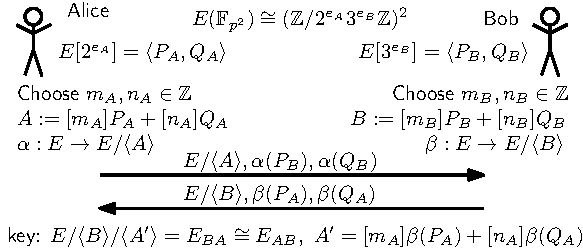
\includegraphics[width = \textwidth]{./sidh.pdf}
    \caption{\label{fig:sidh} The SIDH protocol for $l_A = 2$ and $l_B = 3$.}
\end{figure}

Note that these additional published points $\phi_A(P_B), \phi_A(Q_B), \phi_B(P_A), \phi_B(Q_A)$ make the security assumption required for SIDH somewhat nonstandard.
In particular, it is not enough to assume that the isogeny path problem is hard, and also if we relax this in an analogeous way to the classical Diffie-Hellman assumption (i.e. it is impossible to find $E_{AB}$ given $E_A$ and $E_B$) is not enough.
As it turns out, this additional information indeed decreases the security, as first mentioned by Cristophe Petit \cite{torsion_point_attack}.
However, it still was a big shock when \cite{sidh_broken} discovered an efficient attack using these torsion points, bringing the complete demise of SIDH.
This is even more surprising, as an SIDH-based cryptosystem named SIKE \cite{sike} was already considered a promising candidate for post-quantum crypto, and made it into the fourth (and final) round of the NIST post-quantum standardization process.